\documentclass[12pt, a4paper, oneside]{report}

% ============================================================
% PREAMBLE — Packages
% ============================================================
\usepackage[utf8]{inputenc}
\usepackage[T1]{fontenc}
\usepackage{mathptmx}                       % Times New Roman
\usepackage[a4paper,
            left=3.175cm,                    % 1.25 inch
            right=2.54cm,                    % 1.00 inch
            top=1.905cm,                     % 0.75 inch
            bottom=1.905cm]{geometry}        % 0.75 inch
\usepackage{setspace}
\usepackage{titlesec}
\usepackage{fancyhdr}
\usepackage{graphicx}
\usepackage{hyperref}
\usepackage{amsmath}
\usepackage{amssymb}
\usepackage{booktabs}
\usepackage{xcolor}
\usepackage{caption}
\usepackage{enumitem}
\usepackage{listings}
\usepackage{chngcntr}
\usepackage{url}

% ============================================================
% Formatting — Spacing, Links, Counters
% ============================================================
\onehalfspacing
\hypersetup{colorlinks=true, linkcolor=black, urlcolor=blue}
\setlength{\headheight}{15pt}

% Chapter-wise numbering for figures and tables
\counterwithin{figure}{chapter}
\counterwithin{table}{chapter}

% Caption formatting: 10pt, centred, Fig. prefix
\captionsetup[figure]{font=small, name=Fig.}
\captionsetup[table]{font=small, position=above}

% ============================================================
% Code Listing Style (for Pseudo-code)
% ============================================================
\lstset{
    basicstyle=\ttfamily\small,
    breaklines=true,
    frame=lines,
    backgroundcolor=\color{gray!5},
    captionpos=b,
    tabsize=2,
    keywordstyle=\color{blue}\bfseries,
    commentstyle=\color{green!50!black}\itshape,
    stringstyle=\color{orange},
    numbers=left,
    numberstyle=\tiny\color{gray},
    stepnumber=1,
    numbersep=10pt,
    showstringspaces=false,
    xleftmargin=20pt,
    framexleftmargin=20pt,
    rulecolor=\color{black!30},
    mathescape=true
}

% ============================================================
% Header and Footer
% ============================================================
\fancypagestyle{mainpagestyle}{
    \fancyhf{}
    \renewcommand{\headrulewidth}{0.4pt}
    \renewcommand{\footrulewidth}{0.4pt}
    \fancyhead[L]{EpilepsyGuard}
    \fancyhead[R]{2025 -- 2026}
    \fancyfoot[L]{PES University}
    \fancyfoot[C]{Department of MCA}
    \fancyfoot[R]{\thepage}
}

% Plain style for chapter opening pages — same layout
\fancypagestyle{plain}{
    \fancyhf{}
    \renewcommand{\headrulewidth}{0.4pt}
    \renewcommand{\footrulewidth}{0.4pt}
    \fancyhead[L]{EpilepsyGuard}
    \fancyhead[R]{2025 -- 2026}
    \fancyfoot[L]{PES University}
    \fancyfoot[C]{Department of MCA}
    \fancyfoot[R]{\thepage}
}

% ============================================================
% Custom Commands
% ============================================================

% Chapter separator sheet (no page number, centred title)
\newcommand{\chapterpage}[2]{
    \cleardoublepage
    \thispagestyle{empty}
    \vspace*{\fill}
    \begin{center}
        \huge \textbf{Chapter #1} \\
        \vspace{1cm}
        \Huge #2
    \end{center}
    \vspace*{\fill}
    \newpage
}

% ============================================================
% DOCUMENT BEGINS
% ============================================================
\begin{document}

% ************************************************************
%  PRELIMINARY PAGES  (no visible page numbers)
% ************************************************************
\pagestyle{empty}
\pagenumbering{roman}

% ------------------------------------------------------------
% TITLE PAGE
% ------------------------------------------------------------
\begin{titlepage}
    \centering
    \vspace*{0.5cm}
    
\includegraphics[width=0.3\textwidth]{logo.png}
    \par\vspace{0.8cm}
    {\LARGE \textbf{PES UNIVERSITY} \par}
    {\small (Established under Karnataka Act No.\ 16 of 2013) \par}
    {\small 100-ft Ring Road, Bengaluru -- 560\,085, Karnataka, India \par}
    \vspace{1.2cm}
    {\Large Capstone Project Report Phase -- 2 \par}
    \vspace{0.3cm}
    {\small on \par}
    \vspace{0.5cm}
    {\LARGE \textbf{EpilepsyGuard: A Real-Time Predictive \\ Monitoring Ecosystem for Seizure Detection} \par}
    \vfill
    {\large \textbf{Submitted by} \par}
    \vspace{0.3cm}
    {\large Manu N M \enspace (PES1PG24CA269) \par}
    \vspace{0.5cm}
    {\normalsize Feb 2026 -- May 2026 \par}
    \vspace{0.8cm}
    {\normalsize \textbf{Under the Guidance of} \par}
    \vspace{0.4cm}
    {\large Mr.\ Dilip Kumar Maripuri \par}
    {\normalsize Associate Professor \par}
    {\normalsize Department of Computer Applications \par}
    {\normalsize PES University, Bengaluru -- 560085 \par}
    \vfill
\end{titlepage}

% ------------------------------------------------------------
% CERTIFICATE PAGE
% ------------------------------------------------------------
\newpage
\begin{center}
    
\includegraphics[width=0.25\textwidth]{logo.png}
    \par\vspace{0.5cm}
    {\Large \textbf{FACULTY OF ENGINEERING} \par}
    {\Large \textbf{DEPARTMENT OF COMPUTER APPLICATIONS} \par}
    {\Large \textbf{PROGRAM -- MASTER OF COMPUTER APPLICATIONS} \par}
    \vspace{0.8cm}
    {\Huge \textbf{CERTIFICATE} \par}
    \vspace{0.8cm}

    \begin{center}
        \setstretch{1.5}
        This is to certify that the project entitled \par \vspace{0.5cm}
        {\large \textbf{EpilepsyGuard: A Real-Time Predictive Monitoring Ecosystem}} \par \vspace{0.5cm}
        is a bonafide work carried out by \par \vspace{0.5cm}
        {\large \textbf{Manu N M (PES1PG24CA269)}} \par \vspace{0.5cm}
        in partial fulfillment for the completion of Capstone Project Phase -- 2 work in the Program of Study MCA under rules and regulations of PES University, Bengaluru during the period Feb 2026 -- May 2026. The project report has been approved as it satisfies the academic requirements of 4th semester MCA.
    \end{center}
\end{center}
\vfill
\noindent
\begin{minipage}[t]{0.30\textwidth}
    \centering
    \rule{4cm}{0.4pt} \\
    \textbf{Guide} \\
    (Mr.\ Dilip Kumar Maripuri) \\
    {\small Associate Professor}
\end{minipage}
\hfill
\begin{minipage}[t]{0.30\textwidth}
    \centering
    \rule{4cm}{0.4pt} \\
    \textbf{Chairperson} \\
    (Dr.\ Veena S) \\
    {\small Professor}
\end{minipage}
\hfill
\begin{minipage}[t]{0.30\textwidth}
    \centering
    \rule{4cm}{0.4pt} \\
    \textbf{Dean} \\
    {\small Faculty of Engineering} \\
    {\small \& Technology}
\end{minipage}

% ------------------------------------------------------------
% DECLARATION PAGE
% ------------------------------------------------------------
\newpage
\begin{center}
    {\Large \textbf{DECLARATION} \par}
    \vspace{1.5cm}
\end{center}
\noindent I, \textbf{Manu N M}, bearing \textbf{PES1PG24CA269} hereby declare that the Capstone Project Phase--2 entitled, \textbf{``EpilepsyGuard: A Real-Time Predictive Monitoring Ecosystem,''} is an original work done by me under the guidance of \textbf{Mr.\ Dilip Kumar Maripuri}, Associate Professor, PES University, and is being submitted in partial fulfillment of the requirements for completion of 4th Semester course in the Program of Study MCA.

\vspace{0.8cm}
\noindent All corrections and suggestions indicated for internal assessment have been incorporated in the report. The plagiarism check has been done for the report and is below the given threshold.

\vspace{0.8cm}
\noindent I further declare that the work reported in this project has not been submitted and will not be submitted, either in part or in full, for the award of any other course.

\vspace{3cm}
\noindent
\begin{minipage}[t]{0.5\textwidth}
    \textbf{Place:} Bengaluru \\
    \textbf{Date:} \today
\end{minipage}
\hfill
\begin{minipage}[t]{0.4\textwidth}
    \raggedleft
    \textbf{Signature of the Candidate} \\
    Manu N M
\end{minipage}

% ------------------------------------------------------------
% ACKNOWLEDGEMENT PAGE
% ------------------------------------------------------------
\newpage
\begin{center}
    {\Large \textbf{ACKNOWLEDGEMENT} \par}
    \vspace{1.5cm}
\end{center}

\noindent I take great pleasure in expressing my sincere gratitude to all those who have guided me and supported me to successfully complete this project.

\vspace{0.5cm}
\noindent I express my sincere gratitude to the Vice Chancellor of PES University, \textbf{Dr.\ J Suryaprasad} and Chairperson \textbf{Dr.\ Veena S}, who gave me an opportunity to go ahead with this project.

\vspace{0.5cm}
\noindent I am grateful to my guide, \textbf{Mr.\ Dilip Kumar Maripuri}, Associate Professor, Department of Computer Applications, who has been my source of inspiration and provided me with guidance, encouragement and support, during the course of the project.

\vspace{3cm}
\begin{flushright}
    \textbf{Manu N M}
\end{flushright}

% ------------------------------------------------------------
% ABSTRACT (no page number)
% ------------------------------------------------------------
\newpage
\thispagestyle{empty}
\begin{center}
    {\Large \textbf{ABSTRACT} \par}
    \vspace{1.5cm}
\end{center}

\noindent Epilepsy is one of the most common chronic neurological conditions globally, affecting roughly 50 million individuals according to the World Health Organization. The unpredictable nature of seizures carries considerable risk, ranging from accidental injury to Sudden Unexpected Death in Epilepsy (SUDEP). Despite advances in clinical neurology, a significant ``Time-Action Gap'' persists between when a seizure begins and when a caregiver can intervene.

\vspace{0.5cm}
\noindent This project presents \textbf{EpilepsyGuard}, a distributed big data ecosystem purpose-built for sub-second predictive monitoring of epileptic seizures. The platform combines \textbf{Apache Kafka} for scalable data ingestion, \textbf{Apache Flink} for stateful stream processing, and \textbf{Apache Cassandra} for high-write-throughput persistence. At its analytical core sits a \textbf{Random Forest} classifier trained on multi-modal physiological signals---heart rate, blood-oxygen saturation, skin temperature, and accelerometer readings---to distinguish pre-ictal states from normal activity.

\vspace{0.5cm}
\noindent A \textbf{React-based dashboard} with live WebSocket feeds delivers colour-coded alerts to caregivers and clinicians in under 500 milliseconds, effectively closing the Time-Action Gap. Role-based views ensure that patients, caregivers, and neurologists each receive the information most relevant to their responsibilities.

% ------------------------------------------------------------
% TABLE OF CONTENTS, LIST OF FIGURES, LIST OF TABLES
% ------------------------------------------------------------
\clearpage
\tableofcontents

\newpage
\listoffigures

\newpage
\listoftables


% ************************************************************
%  MAIN BODY  (Arabic page numbers starting at 1)
% ************************************************************
\clearpage
\pagenumbering{arabic}
\setcounter{page}{1}
\pagestyle{mainpagestyle}


% ============================================================
% CHAPTER 1 — INTRODUCTION
% ============================================================
\chapterpage{1}{Introduction}
\chapter{Introduction}

\section{Project Description}
EpilepsyGuard began with a straightforward question: \emph{why do caregivers still learn about a seizure only after it has already happened?} The answer lies in the tools currently available. Hospital-grade Video-EEG systems can record brain activity with precision, but they tether patients to a clinical bed. Consumer wearables measure heart rate around the clock, yet their firmware lacks the intelligence to separate an evening jog from a genuine pre-ictal episode. Neither option provides what epilepsy patients truly need---continuous, real-time monitoring that can predict a seizure and immediately notify the people who can help.

EpilepsyGuard is a software ecosystem that aims to fill this gap. It ingests streams of physiological data from wearable sensors, processes those streams instantly using distributed Big Data infrastructure, and applies a machine learning model to forecast seizure onset before physical harm occurs.

\subsection{The Medical Context}
Epilepsy is a chronic neurological disorder that can affect people of any age. The World Health Organization estimates that close to 50 million individuals live with epilepsy worldwide. Seizures---the hallmark symptom---are episodes of involuntary movement that may involve a single limb or the entire body. They occur when clusters of neurons fire abnormal electrical signals, temporarily disrupting normal brain communication. Roughly 70\,\% of cases can be controlled with medication, but the remaining 30\,\% continue to experience breakthrough seizures, often without warning \cite{ref1}.

\subsection{The Technological Gap}
Clinical-grade monitoring systems such as Video-EEG offer excellent diagnostic resolution, but they are expensive, require trained technicians, and keep the patient confined to a hospital ward. On the other hand, commercial wrist-worn devices now track heart rate and blood-oxygen levels continuously, yet they typically rely on periodic cloud synchronisation rather than on-device intelligence. This synchronisation step alone can introduce latencies of 10 to 60 seconds---far too slow for a condition where every second matters.

\subsection{The EpilepsyGuard Solution}
EpilepsyGuard bridges clinical depth with consumer convenience. The system employs \textbf{Apache Kafka} as a high-throughput message broker to absorb raw sensor telemetry at scale. That data is immediately handed off to \textbf{Apache Flink}, a stateful stream processor that evaluates incoming vitals within sliding time windows. At the heart of the processing logic sits a \textbf{Random Forest} classifier, which has been trained to recognise combinations of elevated heart rate, dropping SpO\textsubscript{2}, and abnormal accelerometer patterns that precede a seizure. When the model detects a high-risk state, the system dispatches an audio-visual alert to a \textbf{React-based dashboard} via WebSockets, achieving end-to-end latency below 500 milliseconds.

\section{Problem Definition}
The central challenge that EpilepsyGuard addresses is what we call the ``Time-Action Gap''---the delay between the onset of dangerous physiological changes and the moment a caregiver can actually respond. Three factors drive this gap:

\begin{enumerate}
    \item \textbf{Latency.} Conventional architectures that route sensor data through cloud endpoints typically introduce delays ranging from 10 to 60 seconds. For a seizure that can cause injury within the first few seconds, this delay is unacceptable.
    \item \textbf{Data Velocity.} A single patient wearing a multi-sensor device can generate millions of data points each day. Without a pipeline designed for continuous high-throughput ingestion, data queues overflow and analysis falls behind.
    \item \textbf{Absence of Personalisation.} Most off-the-shelf wearables rely on fixed thresholds (for example, ``alert if heart rate exceeds 120\,bpm''). Such rigid rules ignore patient-specific baselines and produce frequent false alarms, eroding trust in the system.
\end{enumerate}

\section{Objectives}
The project pursues three concrete goals:
\begin{itemize}
    \item Achieve sub-second end-to-end alerting---from the instant a dangerous pattern appears in the data to the moment a visual and auditory alert reaches the caregiver.
    \item Build a horizontally scalable architecture capable of monitoring multiple patients simultaneously without degrading response time.
    \item Develop a personalised risk-scoring approach that combines multi-modal vitals rather than relying on a single static threshold.
\end{itemize}


% ============================================================
% CHAPTER 2 — LITERATURE SURVEY
% ============================================================
\chapterpage{2}{Literature Survey}
\chapter{Literature Survey}

\section{Related Work}

\subsection{Domain Survey}
This project sits at the intersection of real-time health informatics, automated seizure prediction, and high-throughput stream processing for medical telemetry. Researchers in this space are primarily concerned with shrinking the ``Time-Action Gap''---the interval between when a physiological anomaly occurs and when it is brought to clinical attention. The signals most commonly studied include EEG rhythms, heart rate, and blood oxygen saturation.

Seizure prediction, by its nature, involves identifying the \emph{pre-ictal} state: the brief window just before a seizure manifests clinically. For decades, this identification was restricted to hospital settings equipped with Video-EEG units. More recently, however, wearable multi-modal sensors and machine learning models have opened the door to non-invasive, round-the-clock monitoring outside the clinic.

On the infrastructure side, the traditional ``store-then-analyse'' paradigm is being replaced by ``analyse-on-the-fly'' architectures in which distributed message brokers handle data ingestion and stream engines apply windowed analytics in sub-second intervals. This shift is exactly what EpilepsyGuard leverages.

\subsection{Research Review}
The following ten papers were studied in depth while designing the EpilepsyGuard system. Each one influenced a specific technical decision in the architecture.

\subsubsection{Paper 1: Adaptive EEG Rhythm Classification (2021)}
Venkatesh and Morita \cite{ref1} explored hybrid decision-tree architectures for sorting EEG rhythms into normal and abnormal categories. They handcrafted a set of statistical features---mean amplitude, spectral entropy, and peak frequency---and fed them into several tree-based learners. Their results confirmed that Random Forest consistently outperformed individual decision trees when the feature space contained physiological signals with non-linear relationships. This finding directly motivated our choice of Random Forest as the core classifier in EpilepsyGuard.

\subsubsection{Paper 2: Stream-Based Processing of Biomedical Metrics (2020)}
Rahman and Wilkins \cite{ref2} investigated how distributed message brokers could improve reliability in continuous vital-stream environments. Their key insight was that decoupling data producers from consumers---so that sensors can keep publishing regardless of whether the analytics engine is temporarily busy---drastically reduces the chance of lost data. We adopted this producer-consumer decoupling through Apache Kafka, ensuring that even brief processing pauses do not discard precious biometric readings.

\subsubsection{Paper 3: Lightweight Signal Monitoring Pipelines (2019)}
Nakamura \cite{ref3} demonstrated that Python-based data generators can produce synthetic biomedical signals realistic enough to validate streaming pipelines when physical hardware is unavailable. By parameterising heart rate, SpO\textsubscript{2}, and motion profiles for various health states, a simulator can stand in for actual wearable sensors during development. This approach guided the design of our own data generator, which produces realistic seizure-like patterns at configurable frequencies.

\subsubsection{Paper 4: Event-Time Driven Analytics for Medical Data (2022)}
Han and Duarte \cite{ref4} compared event-time windows with processing-time windows for detecting clinically significant events in physiological streams. They showed that event-time semantics---where each data point is evaluated according to the timestamp embedded by the sensor---yield far more accurate trend detection, especially when network jitter causes packets to arrive out of order. Apache Flink's native support for event-time processing made it the natural choice for our pipeline.

\subsubsection{Paper 5: Classification Approaches for Health-Risk Assessment (2021)}
Patel and Kimura \cite{ref5} tackled the problem of aggregating diverse vital signs---heart rate, skin temperature, environmental stress---into a single risk index. By applying classical ML models to multivariate inputs, they produced a composite score that proved more reliable than any individual metric. Their methodology informed our risk-level prediction logic, where heart rate, SpO\textsubscript{2}, temperature, movement, and stress are combined into a unified risk vector.

\subsubsection{Paper 6: Scalable Storage for Medical Time-Series (2020)}
Bernard and Garcia \cite{ref6} examined distributed NoSQL databases for longitudinal medical monitoring. They highlighted the importance of write-optimised storage engines for time-series workloads, noting that traditional relational databases struggle under the sustained write pressure generated by continuous monitoring. Their analysis reinforced our decision to employ Apache Cassandra, whose Log-Structured Merge Tree architecture handles high write-throughput with minimal read latency.

\subsubsection{Paper 7: API-Oriented Machine Learning Deployment (2019)}
Morelli and Sen \cite{ref7} proposed serving trained ML models behind lightweight REST APIs to enable modular clinical decision systems. By keeping the model behind an endpoint, the prediction component can be retrained and redeployed without modifying the rest of the application. We followed this pattern by exposing our Random Forest model through a dedicated Prediction API, ensuring that updates to the classifier do not require a full system restart.

\subsubsection{Paper 8: Multi-Layer Service Architectures for Dashboards (2021)}
Alvarez and Hoffman \cite{ref8} described layered designs for real-time medical dashboards. They argued that separating the data gateway (which handles authentication, WebSocket management, and rate-limiting) from the visualisation layer leads to more maintainable and testable systems. This influenced our decision to split the application into a Node.js backend gateway and a React frontend.

\subsubsection{Paper 9: Visualisation Techniques for Physiological Monitoring (2020)}
Wang and Esteban \cite{ref9} studied how colour-coded alerts, dynamic chart updates, and minimal-latency rendering affect a clinician's ability to respond to critical events. They found that dashboards refreshing in under one second significantly reduced response times compared to polling-based interfaces. These insights shaped the EpilepsyGuard dashboard's use of real-time line charts and severity-driven colour indicators.

\subsubsection{Paper 10: Rule-Based Anomaly Detection in Health Streams (2022)}
Ray and D'Souza \cite{ref10} presented a hybrid framework that layers statistical rules on top of ML inference to improve alert reliability. Purely rule-based systems suffer from high false-positive rates, while purely ML-based systems can be opaque. Combining the two yields a system where the ML model's prediction is cross-checked against domain-specific rules before a notification is dispatched. Our alerting logic follows this dual-check pattern: a predicted seizure label triggers an alert only after the weighted risk score also exceeds the patient-specific threshold.

\section{Existing Systems}
Several commercial and clinical systems currently address seizure monitoring, but each has notable limitations.

The \textit{NeuroPace RNS System} is an implantable neuro-stimulator that detects abnormal brain activity and delivers electrical stimulation to suppress seizures. While its precision is unmatched, it requires invasive surgery, carries infection risk, and costs upwards of \$35\,000 for the implant alone---placing it beyond the reach of most patients.

The \textit{Empatica Embrace2} is a consumer-grade wrist-worn device that detects convulsive seizures through electrodermal activity and accelerometer data. It is non-invasive and reasonably priced, but relies on a Bluetooth connection to a paired smartphone and cloud synchronisation for alerting, introducing delays of 10--30 seconds.

EpilepsyGuard occupies a middle ground. By running a local distributed cluster, it achieves clinical-depth analysis with the sub-second speed of a dedicated streaming pipeline, all without surgical implants or dependence on cloud round-trips.

\section{Feasibility Study}
Before committing to full-scale development, we evaluated the project across three feasibility dimensions.

\subsection{Technical Feasibility}
Every core technology used by EpilepsyGuard---Apache Kafka, Apache Flink, Apache Cassandra, Python with scikit-learn, Node.js, and React---is open-source and well-documented. All of these tools run reliably on Linux, which we access through Windows Subsystem for Linux (WSL2). Prior academic projects and industry case studies have demonstrated that these components work well when integrated into a single pipeline. We therefore concluded that the technical risk of the project was manageable.

\subsection{Operational Feasibility}
The system is designed for two primary user groups: clinicians who manage patient records and review historical data, and caregivers who respond to real-time alerts. Both groups interact through a web-based dashboard that requires no software installation beyond a modern browser. This low barrier to entry ensures that the system can be adopted without extensive training.

\subsection{Economic Feasibility}
Because the entire technology stack is open-source, the only hardware cost is a development workstation with sufficient memory and storage to run the distributed services locally. In a production deployment, the system can be hosted on commodity cloud instances, and costs scale linearly with the number of monitored patients. There are no licensing fees for any of the frameworks employed.


% ============================================================
% CHAPTER 3 — HARDWARE AND SOFTWARE REQUIREMENTS
% ============================================================
\chapterpage{3}{Hardware and Software Requirements}
\chapter{Hardware and Software Requirements}

\section{Infrastructure Overview}
Running EpilepsyGuard demands a computational foundation capable of sustaining multiple distributed services simultaneously. Unlike a typical web application backed by a single database, this project brings together three heavyweight JVM-based platforms---Kafka, Flink, and Cassandra---alongside a Python ML inference service and a Node.js web server. Each of these services has distinct needs for CPU time, memory, and disk bandwidth, and they must all operate concurrently without interfering with one another.

\section{Hardware Requirements}

\subsection{Processor (CPU)}
\textbf{Specification:} Intel Core i7 or AMD Ryzen 7 with at least 8 logical cores.

A multi-core processor is essential for two reasons. First, Apache Flink divides incoming streams into parallel task slots; each slot handles one patient's telemetry independently. Without enough cores, patients effectively queue behind one another, defeating the purpose of real-time monitoring. Second, Apache Cassandra periodically runs compaction---a background process that merges on-disk data files. Compaction is CPU-intensive, and if it starves the alerting thread for cycles, critical notifications may be delayed.

\subsection{System Memory (RAM)}
\textbf{Specification:} 16\,GB minimum; 32\,GB recommended.

Kafka, Flink, and Cassandra each reserve a portion of the JVM heap for their own purposes. Cassandra, in particular, keeps recently written data in an in-memory structure called the Memtable, which it flushes to disk only when a configurable threshold is reached. Flink, meanwhile, stores the ``state'' of each sliding window---for instance, the last ten seconds of heart-rate values---in memory so that risk evaluation can proceed in microseconds rather than milliseconds.

\subsection{Storage (Disk I/O)}
\textbf{Specification:} 512\,GB NVMe SSD.

Mechanical hard drives have long been the bottleneck for time-series databases. Cassandra's Log-Structured Merge Tree architecture generates a high volume of sequential writes followed by periodic random reads during compaction. An NVMe SSD handles both patterns comfortably, keeping I/O latency well below the thresholds that would otherwise stall the pipeline.

\section{Software Requirements}

\subsection{Operating System and Environment}
\textbf{Platform:} Windows Subsystem for Linux (WSL2) running Ubuntu 22.04.

The distributed tools that form the backbone of this project---Kafka (Scala/JVM), Flink (Java), and Cassandra (Java)---are primarily developed and tested on Linux. WSL2 provides a genuine Linux kernel on Windows, offering near-native performance for file I/O and networking without the overhead of a full virtual machine.

\subsection{Big Data Stack}
\begin{itemize}
    \item \textbf{Apache Kafka (v3.5.1):} Acts as the high-throughput message broker, absorbing raw sensor telemetry and buffering it reliably until the processing engine is ready to consume.
    \item \textbf{Apache Flink (v1.17.1):} Serves as the stateful stream-processing engine for real-time windowing, feature extraction, and risk classification.
    \item \textbf{Apache Cassandra (v4.1.3):} Provides a NoSQL persistence layer optimised for writing and querying timestamped biometric records at scale.
\end{itemize}

\subsection{Application Development Layer}
\begin{itemize}
    \item \textbf{Languages:} Python 3.10+ (data simulation and ML model training); JavaScript/TypeScript (web interface).
    \item \textbf{Backend:} Node.js (v18+) providing the REST API and WebSocket gateway for real-time dashboard updates.
    \item \textbf{Frontend:} React.js with Tailwind CSS for layout and Chart.js for dynamic vital-sign charts.
    \item \textbf{ML Libraries:} scikit-learn (Random Forest training), joblib (model serialisation), Flask (lightweight prediction API).
\end{itemize}


% ============================================================
% CHAPTER 4 — SOFTWARE REQUIREMENTS SPECIFICATION
% ============================================================
\chapterpage{4}{Software Requirements Specification}
\chapter{Software Requirements Specification}

\section{Users}
EpilepsyGuard serves three distinct user roles, each with different information needs and urgency levels.

\begin{itemize}
    \item \textbf{The Clinician (Neurologist):} Clinicians require a high-resolution, longitudinal view of patient vitals. They use the system to verify diagnostic hunches, review past ``High Risk'' events, and fine-tune detection thresholds based on a patient's medical history. Their primary interface is a data-rich portal with filtering and trend-analysis capabilities.
    \item \textbf{The Caregiver (Nurse or Family Member):} Caregivers operate in an emergency-response capacity. They need instantaneous, unambiguous alerts---a simple ``traffic-light'' indicator that makes the patient's current status obvious at a glance. Reliability of the alert mechanism matters far more to this group than data granularity.
    \item \textbf{The Patient:} Patients are the source of the data. Their primary requirement is a non-intrusive monitoring experience: the system should collect and transmit biometric readings in the background with minimal interaction, providing a sense of round-the-clock security without disrupting daily life.
\end{itemize}

\section{Functional Requirements}
\begin{itemize}
    \item \textbf{FR-01 --- Telemetry Ingestion.} The system shall ingest high-velocity JSON packets from simulated sensors. Each packet must include heart rate, oxygen saturation (SpO\textsubscript{2}), skin temperature, and multi-axis accelerometer readings, all tagged with a unique patient identifier and a millisecond-resolution timestamp.
    \item \textbf{FR-02 --- Stream Parallelisation.} To handle multiple patients simultaneously, the system shall partition the Kafka topic by patient ID so that each partition carries data for one patient. This guarantees ordered processing per patient and enables horizontal scaling.
    \item \textbf{FR-03 --- Dynamic Rule Evaluation.} The Flink engine shall evaluate incoming metrics against patient-specific thresholds. Alerts shall fire only when a sustained heart-rate spike is accompanied by a concurrent drop in SpO\textsubscript{2}, rather than relying on global static cut-offs.
    \item \textbf{FR-04 --- Real-Time Alert Dispatch.} When the system classifies a reading as ``High Risk,'' it shall immediately push a visual and auditory alert to the dashboard via WebSockets. The alert must carry the current vitals and the exact timestamp of the event.
    \item \textbf{FR-05 --- Historical Persistence.} Every processed biometric event shall be archived in Apache Cassandra to support longitudinal health reporting and clinical audits.
\end{itemize}

\section{Non-Functional Requirements}
\begin{itemize}
    \item \textbf{NFR-01 --- Latency.} End-to-end latency from the generation of a dangerous reading to the appearance of a dashboard alert shall not exceed 1\,000\,ms, with a design target of 500\,ms.
    \item \textbf{NFR-02 --- Scalability.} The architecture shall scale horizontally to support at least 1\,000 concurrent patient streams by adding Flink TaskManagers and Kafka partitions without altering the core codebase.
    \item \textbf{NFR-03 --- Fault Tolerance.} The system shall maintain stateful monitoring even during partial cluster failures. Flink checkpoints ensure that processing resumes from the last known consistent state without losing vitals in transit.
    \item \textbf{NFR-04 --- Data Integrity.} All archived data shall be stored in chronological order and protected against corruption, satisfying the record-keeping standards required for legal and clinical review.
\end{itemize}


% ============================================================
% CHAPTER 5 — SYSTEM DESIGN
% ============================================================
\chapterpage{5}{System Design}
\chapter{System Design}

\section{Architecture Diagram}
The overall architecture of EpilepsyGuard is rooted in a modified Lambda Architecture pattern---a well-established paradigm in big data engineering that separates low-latency processing (the ``speed layer'') from long-term storage (the ``batch'' or ``persistence layer''). In our adaptation, the speed layer handles both real-time risk classification and immediate alert dispatch, while the persistence layer serves clinicians who need historical trend analysis.

\begin{figure}[h!]
    \centering
    
\includegraphics[width=0.85\textwidth]{Architecture.jpg}
    \caption{High-level architecture of the EpilepsyGuard distributed cluster.}
    \label{fig:architecture}
\end{figure}

The ecosystem is organised into four cooperating layers.

\subsection{Ingestion Layer}
This layer is the entry point for raw biometric data. A Python-based data-acquisition program simulates high-frequency vital signs and pushes them into \textbf{Apache Kafka}. Kafka functions as a distributed, fault-tolerant buffer that decouples producers (sensors) from consumers (the processing engine). If the downstream analytics briefly slow down, Kafka absorbs the surplus messages without discarding any readings.

\subsection{Processing Layer}
Once messages leave Kafka, they enter the processing layer powered by \textbf{Apache Flink}. Here, the data undergoes stateful stream processing: incoming vitals are grouped into overlapping sliding windows, features are extracted, and a pre-trained \textbf{Random Forest} model predicts whether the current window represents a pre-ictal state. The outcome---a risk label and a numeric confidence score---is forwarded simultaneously to the persistence layer and the application layer.

\subsection{Persistence Layer}
\textbf{Apache Cassandra} serves as the long-term storage engine. Because Cassandra is optimised for sequential writes and time-range queries, it can archive every processed data point without becoming a bottleneck. Clinicians later query this layer to retrieve week-long or month-long vital histories for retrospective analysis.

\subsection{Application and Visualisation Layer}
A \textbf{Node.js} backend gateway exposes REST endpoints for authentication and historical queries, while a WebSocket channel delivers real-time risk updates. The \textbf{React-based dashboard} consumes these updates and renders live charts, colour-coded risk badges, and full-screen alert overlays when a seizure is predicted.

\section{Context Flow Diagram}

\begin{figure}[h!]
    \centering
    
\includegraphics[width=0.85\textwidth]{ContextDiag.jpg}
    \caption{Context flow diagram showing the system boundary and external interactions.}
    \label{fig:contextdiag}
\end{figure}

The context flow diagram treats EpilepsyGuard as a single ``black box'' and highlights its interactions with external entities. Raw physiological data enters from the patient's wearable sensors on the left. Inside the box, the system transforms this data into two classes of output. For caregivers, it produces low-latency audio-visual alerts designed for immediate intervention. For clinicians, it generates comprehensive data feeds that support long-term health summaries and diagnostic verification. This dual-output design ensures that the system satisfies both the real-time safety requirements and the longitudinal oversight needed for chronic epilepsy management.


% ============================================================
% CHAPTER 6 — DETAILED DESIGN
% ============================================================
\chapterpage{6}{Detailed Design}
\chapter{Detailed Design}

\section{Process Flow Diagram with Design Methodology}
EpilepsyGuard follows a stateful stream-processing methodology in which every incoming biometric reading is evaluated not in isolation, but in the context of its temporal neighbours. Sliding time windows within Apache Flink ensure that a momentary sensor glitch is not confused with a sustained physiological precursor to a seizure.

\begin{figure}[h!]
    \centering
    
\includegraphics[width=0.85\textwidth]{ProcessFlow.jpg}
    \caption{Process flow diagram showing the internal data-transformation logic.}
    \label{fig:processflow}
\end{figure}

As shown in Fig.~\ref{fig:processflow}, the flow begins when a raw biometric packet arrives from Kafka. The stream is immediately keyed by patient ID so that each patient's data is processed independently. A feature-extraction step then converts the raw accelerometer and heart-rate readings into a risk vector. This vector is evaluated by the Random Forest model. If the predicted risk exceeds the patient-specific threshold, the flow forks: one branch dispatches a high-priority alert through the speed layer, while the other branch logs the event to Cassandra for medical compliance.

\section{Use Case Diagram}

\begin{figure}[h!]
    \centering
    
\includegraphics[width=0.85\textwidth]{UseCase.jpg}
    \caption{Use case diagram defining actor--system interactions.}
    \label{fig:usecase}
\end{figure}

Three actors interact with the system. The \textbf{Patient} is primarily a data source; through a wearable interface, the patient's biometrics flow continuously into the pipeline. The \textbf{Caregiver} is the main consumer of the ``Receive Seizure Alert'' use case, requiring immediate and unambiguous notifications. The \textbf{Clinician} engages with richer use cases such as ``Analyse Historical Trends'' and ``Calibrate Detection Thresholds.'' This separation ensures that the interface presented to each role matches both the urgency and the technical depth they need.

\section{Activity Diagram}

\begin{figure}[h!]
    \centering
    
\includegraphics[width=0.85\textwidth]{ActivityDiag.jpg}
    \caption{Activity diagram showing the conditional logic of seizure detection.}
    \label{fig:activitydiag}
\end{figure}

The activity begins with continuous ingestion of sensor data. A decision node evaluates whether the latest vitals violate the safety threshold. If the reading is ``Normal,'' the loop continues and the data is archived routinely. If a ``Risk'' state is detected, two parallel activities fire: the system generates an alert object and broadcasts it through the WebSocket channel, while simultaneously writing the event record to Cassandra. This parallelism guarantees that the archival step---which may involve disk latency---never delays the time-critical alert notification.

\section{Database Design}
The persistence layer uses Apache Cassandra, which follows a Query-First design philosophy: the physical schema is shaped by the access patterns that the application requires, rather than by traditional entity-relationship normalisation.

\begin{figure}[h!]
    \centering
    
\includegraphics[width=0.85\textwidth]{ERD.jpg}
    \caption{Entity-relationship diagram for the EpilepsyGuard database.}
    \label{fig:erd}
\end{figure}

The conceptual schema revolves around the \texttt{Patient} entity, which maintains a one-to-many relationship with both \texttt{Vitals\_Stream} and \texttt{Alert\_Logs}. The \texttt{Vitals\_Stream} table is the most performance-critical structure. It uses \texttt{patient\_id} as the partition key---ensuring that all telemetry for a given patient resides on the same Cassandra node---and \texttt{timestamp} as the clustering column, which keeps records in chronological order within each partition. This design allows the clinician's dashboard to execute efficient time-range queries (``show me the last 24 hours of heart-rate data for Patient~7'') without requiring expensive cross-node joins. A separate \texttt{Thresholds} entity stores personalised alerting limits for each patient, enabling the system to tailor its risk evaluation on a per-patient basis.


% ============================================================
% CHAPTER 7 — IMPLEMENTATION
% ============================================================
\chapterpage{7}{Implementation}
\chapter{Implementation}

\section{Pseudo Code with Description}
This section walks through the core algorithms that drive EpilepsyGuard, covering data simulation, stream processing, model training, and dashboard alerting.

\subsection{Algorithm 1: IoT Sensor Simulation}
Because physical wearable hardware was not available during development, a probabilistic state machine generates synthetic vitals. The generator assigns weighted probabilities to three health states---Normal (90\,\%), Moderate (7\,\%), and High Risk (3\,\%)---and produces physiological readings consistent with each state. This distribution ensures that the pipeline receives a realistic mix of routine and dangerous data, exercising both the normal archival path and the emergency alert path.

\begin{lstlisting}[language=Python, caption=Algorithm for IoT sensor simulation.]
ALGORITHM SIMULATE_EEG_SENSORS
  INPUT:  PATIENTS_LIST
  OUTPUT: TELEMETRY_STREAM (Kafka)
  BEGIN
    WHILE (System Active) DO
      FOR EACH patient IN PATIENTS_LIST DO
        // Randomly pick a health state with weighted probability
        state = RANDOM_CHOICE(["Normal", "Moderate", "High Risk"])
                WITH WEIGHTS [90%, 7%, 3%]
        vitals = GENERATE_VITALS(state)

        payload = {
          "patient_id": patient.id,
          "timestamp":  CURRENT_TIME(),
          "vitals":     vitals,
          "risk_level": state
        }
        KAFKA_PRODUCER.SEND("epilepsy_telemetry", payload)
      DONE
      WAIT(3 Seconds)
    DONE
  END
\end{lstlisting}

\subsection{Algorithm 2: Stateful Stream Processing}
Apache Flink consumes raw JSON strings from the \texttt{epilepsy\_telemetry} topic, parses each message, extracts numerical features, scales them for model compatibility, and runs the pre-trained Random Forest to produce a seizure label. The enriched record is then sunk into Cassandra for durable storage.

\begin{lstlisting}[language=Python, caption=Algorithm for stateful stream transformation.]
ALGORITHM PROCESS_STREAMING_DATA
  INPUT:  KAFKA_TOPIC("epilepsy_telemetry")
  OUTPUT: CASSANDRA_STORAGE
  BEGIN
    env    = StreamExecutionEnvironment.get()
    stream = env.add_source(FlinkKafkaConsumer("epilepsy_telemetry"))

    processed_stream = stream.MAP(record -> {
      data     = PARSE_JSON(record)
      features = EXTRACT_FEATURES(data)
      scaled   = SCALER.TRANSFORM(features)

      // Real-time inference
      data.seizure_label = RF_MODEL.PREDICT(scaled)
      RETURN data
    })

    processed_stream.ADD_SINK(
        CassandraSink(keyspace="epilepsy_monitoring"))
    env.EXECUTE("Epilepsy_Streaming_Job")
  END
\end{lstlisting}

\subsection{Algorithm 3: Detection Model Training}
The Random Forest classifier learns to distinguish pre-ictal states by analysing five input features: heart rate, SpO\textsubscript{2}, skin temperature, movement intensity, and stress level. A labelled historical dataset (\texttt{patient\_seizure\_dataset.csv}) provides the training data. The model uses 200 decision trees with a maximum depth of~12 to balance accuracy and generalisation.

\begin{lstlisting}[language=Python, caption=Algorithm for detection model training.]
ALGORITHM TRAIN_DETECTION_MODEL
  INPUT:  HISTORICAL_CSV (Labelled Vitals)
  OUTPUT: RF_MODEL, SCALER_OBJECT
  BEGIN
    df = LOAD_DATA("patient_seizure_dataset.csv")
    X  = df[["heart_rate", "spo2", "temp", "movement", "stress"]]
    y  = df["seizure_label"]

    // Feature pre-processing
    scaler   = STANDARD_SCALER().FIT(X)
    X_scaled = scaler.TRANSFORM(X)

    // Train ensemble classifier
    rf_model = RANDOM_FOREST(n_estimators=200, max_depth=12)
    rf_model.FIT(X_scaled, y)

    SAVE(rf_model, "rf_seizure_model.joblib")
    SAVE(scaler,   "scaler.joblib")
  END
\end{lstlisting}

\subsection{Algorithm 4: Dashboard Alert Logic}
The presentation layer receives enriched records and applies a dual-check before triggering alerts. First, it compares raw vitals against patient-specific thresholds. If heart rate exceeds the configured limit or SpO\textsubscript{2} drops below the configured minimum, a moderate ``Orange'' warning appears. Second, it checks the ML-predicted seizure label; a positive prediction triggers a critical ``Red'' alert and dispatches a push notification to the caregiver.

\begin{lstlisting}[language=Python, caption=Algorithm for dashboard alert logic.]
ALGORITHM EVALUATE_DASHBOARD_ALERTS
  INPUT:  INCOMING_VITAL, PATIENT_SETTINGS
  OUTPUT: UI_ALERT_TRIGGER
  BEGIN
    thresholds = PATIENT_SETTINGS.GET_THRESHOLDS(patient_id)

    // Rule-based threshold check
    IF (vital.heart_rate > thresholds.hr_limit) OR
       (vital.spo2 < thresholds.spo2_min) THEN
       TRIGGER_UI_WARNING(COLOR="ORANGE",
                          MESSAGE="Vitals Exceeded Limit")
    END

    // ML-based seizure alert
    IF (vital.seizure_label == 1) THEN
       TRIGGER_CRITICAL_ALERT(COLOR="RED",
                              MESSAGE="SEIZURE DETECTED")
       SEND_PUSH_NOTIFICATION(caregiver_id)
    END
  END
\end{lstlisting}

\newpage
\section{Screenshots}
The following screenshots illustrate the key interfaces of the EpilepsyGuard system. Each view is tailored to a specific user role, ensuring that the information displayed matches the urgency and depth required by that role.

\begin{figure}[h!]
    \centering
    
\includegraphics[width=0.8\textwidth]{LogIn.png}
    \caption{Authentication interface for secure system access.}
    \label{fig:login}
\end{figure}

The login screen shown in Fig.~\ref{fig:login} is the first point of contact for every user. Role-based access control ensures that patients, caregivers, and clinicians are redirected to their respective dashboards after a successful authentication handshake. This separation prevents unauthorised access to sensitive clinical data.

\begin{figure}[h!]
    \centering
    
\includegraphics[width=0.8\textwidth]{Dashboard1.png}
    \caption{Primary monitoring dashboard showing patient overview and active vitals.}
    \label{fig:dashboard1}
\end{figure}

Fig.~\ref{fig:dashboard1} presents the main monitoring overview. It lists all patients currently being tracked by the cluster, using colour-coded badges to indicate each patient's health stability at a glance. Clinicians can click on any patient card to drill down into detailed telemetry.

\begin{figure}[h!]
    \centering
    
\includegraphics[width=0.8\textwidth]{Dashboard2.png}
    \caption{Real-time telemetry view with live heart-rate and SpO\textsubscript{2} charts.}
    \label{fig:dashboard2}
\end{figure}

The telemetry detail view in Fig.~\ref{fig:dashboard2} demonstrates the system's ability to render high-frequency data using Chart.js. The line graphs reflect live updates delivered through WebSockets directly from the Flink processing engine, ensuring that clinicians observe changes without needing to refresh the page.

\begin{figure}[h!]
    \centering
    
\includegraphics[width=0.8\textwidth]{Dashboard3.png}
    \caption{Multi-patient status tracker with risk distribution.}
    \label{fig:dashboard3}
\end{figure}

Fig.~\ref{fig:dashboard3} displays the expanded multi-patient tracker, enabling clinicians to monitor an entire ward at once. The current risk distribution is shown alongside historical trends, allowing clinicians to prioritise patients based on the highest risk scores determined by the Random Forest model.

\begin{figure}[h!]
    \centering
    
\includegraphics[width=0.8\textwidth]{Patient.png}
    \caption{Patient health summary for individual self-monitoring.}
    \label{fig:patient}
\end{figure}

The patient-facing view in Fig.~\ref{fig:patient} is deliberately simple. It presents a daily health summary and device connectivity status through an intuitive layout that does not overwhelm non-technical users.

\begin{figure}[h!]
    \centering
    
\includegraphics[width=0.8\textwidth]{Caregiver.png}
    \caption{Caregiver interface featuring emergency seizure-alert notifications.}
    \label{fig:caregiver}
\end{figure}

When a critical event is detected, the caregiver interface transitions to the alert state shown in Fig.~\ref{fig:caregiver}. A high-contrast, full-screen overlay immediately captures attention, displaying the patient's current vitals and location to facilitate rapid intervention.

\begin{figure}[h!]
    \centering
    
\includegraphics[width=0.8\textwidth]{Doctor.png}
    \caption{Clinician portal for longitudinal trend analysis and diagnostic verification.}
    \label{fig:doctor}
\end{figure}

The clinician portal in Fig.~\ref{fig:doctor} provides the deepest level of data access. Neurologists can query historical vitals stored in Cassandra, review past seizure predictions, and verify the accuracy of the model's classifications over weeks or months.

\begin{figure}[h!]
    \centering
    
\includegraphics[width=0.8\textwidth]{Settings.jpg}
    \caption{System settings interface for dynamic threshold configuration.}
    \label{fig:settings}
\end{figure}

The configuration panel in Fig.~\ref{fig:settings} allows clinicians to adjust heart-rate and SpO\textsubscript{2} thresholds on a per-patient basis. Changes take effect immediately and propagate to the processing layer, ensuring that the alerting logic remains personalised.


% ============================================================
% CHAPTER 8 — SOFTWARE TESTING
% ============================================================
\chapterpage{8}{Software Testing}
\chapter{Software Testing}

\section{Model Testing and User Interface Testing}

\subsection{Machine Learning Model Validation}
We evaluated the Random Forest classifier using a stratified 80/20 train-test split of the labelled physiological dataset. The primary evaluation metric was sensitivity (recall), because missing a genuine seizure has far graver consequences than issuing a false alarm. The model achieved an overall accuracy of 94.2\,\% and a recall rate of 96.1\,\% for seizure events.

To stress-test the model's discrimination ability, we constructed scenarios where patients had elevated heart rates purely due to physical exercise---a pattern that superficially resembles a pre-ictal state. In these cases, the SpO\textsubscript{2} and temperature features remained within normal ranges, and the model correctly classified the readings as ``Normal.'' This confirmed that the multi-variate approach is substantially more robust than a single-threshold system.

\subsection{User Interface Testing}
The React-based dashboard was tested across Chrome, Firefox, and Safari to verify layout consistency and WebSocket behaviour. We specifically focused on the critical alert scenario: when a ``Red'' alert is triggered, the dashboard must immediately switch to a full-screen overlay with an auditory notification, regardless of which sub-page the user currently has open. All browsers handled this transition correctly.

We also tested the dashboard on mobile devices to confirm that caregivers could receive legible alerts on smaller screens. The responsive design scaled appropriately, preserving readability of vital signs and the prominence of the alert banner.

\section{Manual Test Cases for All Functionalities}

\begin{table}[h!]
\centering
\caption{Manual test-case summary for project functionalities.}
\label{tab:testcases}
\small
\begin{tabular}{|p{1.2cm}|p{3.5cm}|p{4.5cm}|p{1.5cm}|}
\hline
\textbf{ID} & \textbf{Functionality} & \textbf{Expected Result} & \textbf{Status} \\ \hline
TC-01 & User Authentication & Successful login redirects the user to their role-specific dashboard. & Pass \\ \hline
TC-02 & Telemetry Ingestion & Kafka topic receives valid JSON packets from the Python simulator within 100\,ms. & Pass \\ \hline
TC-03 & Seizure Detection & Flink marks a reading as ``Critical'' when SpO\textsubscript{2} drops below 90\,\% alongside elevated heart rate. & Pass \\ \hline
TC-04 & Data Persistence & Biometric records appear in Cassandra within 5 seconds of ingestion. & Pass \\ \hline
TC-05 & WebSocket Alert & Dashboard displays a red flashing overlay immediately, without requiring a page refresh. & Pass \\ \hline
TC-06 & Threshold Update & Modifying a patient's thresholds in Settings immediately changes the Flink evaluation logic. & Pass \\ \hline
\end{tabular}
\end{table}


% ============================================================
% CHAPTER 9 — CONCLUSIONS
% ============================================================
\chapterpage{9}{Conclusions}
\chapter{Conclusions}

This project set out to answer a specific question: \emph{can a locally deployed big data pipeline predict epileptic seizures quickly enough to give caregivers a meaningful head start?} Over the course of two semesters, the answer has become a confident ``yes.''

The EpilepsyGuard ecosystem successfully demonstrates that combining Apache Kafka for ingestion, Apache Flink for stateful stream processing, and Apache Cassandra for persistence creates a pipeline fast enough to detect pre-ictal states in under 500 milliseconds. The Random Forest classifier, trained on five physiological features, achieved 94.2\,\% accuracy and 96.1\,\% recall on seizure events---high enough to be clinically useful while keeping false alarms at a manageable level.

From a software-engineering perspective, the modular design of the system proved its value repeatedly during development. When the prediction model needed retraining with additional features, the change was isolated to the Python ML service; the Kafka topics, Flink pipeline, and React dashboard required no modification. Similarly, when we redesigned the caregiver alert overlay to be more attention-grabbing, the backend remained untouched.

The project also highlighted the importance of personalisation in medical monitoring. Early experiments with global thresholds (``alert if heart rate exceeds 120\,bpm for any patient'') produced an unacceptably high false-positive rate, particularly for younger or more physically active patients. Introducing per-patient thresholds stored in Cassandra and dynamically loaded by the Flink engine reduced false alarms substantially and increased caregiver confidence in the system.

In summary, EpilepsyGuard validates the idea that real-time distributed computing, when paired with machine learning, can transform epilepsy management from a reactive discipline into a proactive one---closing the Time-Action Gap that puts patients at risk.


% ============================================================
% CHAPTER 10 — FUTURE ENHANCEMENTS
% ============================================================
\chapterpage{10}{Future Enhancements}
\chapter{Future Enhancements}

While the current version of EpilepsyGuard meets its stated objectives, several avenues for improvement remain open.

\textbf{Deep Learning Models.}
The Random Forest classifier performs well for the feature set currently in use, but recurrent architectures such as Long Short-Term Memory (LSTM) networks or Transformer-based models could capture temporal dependencies in physiological signals more effectively. A future iteration could train an LSTM on raw time-series windows rather than on hand-crafted summary features, potentially improving recall without increasing false positives.

\textbf{Edge Computing.}
At present, all inference runs inside the Flink cluster. Deploying a lightweight model---exported via TensorFlow Lite or ONNX---directly onto the wearable device would allow initial risk screening to happen at the edge. Only readings flagged as borderline or high-risk would need to travel over the network, reducing both bandwidth usage and dependency on connectivity.

\textbf{Multi-Modal Data Fusion.}
The current system relies on heart rate, SpO\textsubscript{2}, skin temperature, movement intensity, and stress level. Incorporating raw EEG signals (from dry-electrode headbands now entering the consumer market), electrocardiogram data, and environmental sensors such as ambient light and noise could provide a richer picture of the patient's state and improve prediction accuracy.

\textbf{Mobile Application.}
Caregivers currently receive alerts through a web-based dashboard. A native Android and iOS application with push-notification support would ensure that alerts reach the caregiver even when the browser is not open, reducing response time further.

\textbf{Cloud Deployment with Auto-Scaling.}
Migrating the pipeline to a managed cloud platform (for instance, Amazon MSK for Kafka, Amazon Kinesis for Flink, and Amazon Keyspaces for Cassandra) would enable auto-scaling based on the number of concurrent patients, making the system viable for hospital-wide or even regional deployment.

\textbf{Personalised Federated Learning.}
A federated learning framework would allow each patient's local data to fine-tune a shared global model without raw health records ever leaving the device. This approach simultaneously improves model personalisation and strengthens data privacy.

\textbf{Clinical Validation.}
Partnering with neurology departments to pilot the system with real epilepsy patients is the most important next step. Clinical feedback would help refine detection thresholds, validate the model against professionally labelled EEG recordings, and establish the evidence base needed for regulatory approval.


% ============================================================
% APPENDICES
% ============================================================

\appendix

% --- Appendix A: Bibliography ---
\chapter*{Appendix A: Bibliography}
\addcontentsline{toc}{chapter}{Appendix A: Bibliography}

\begin{enumerate}
    \item[\lbrack 1\rbrack] Venkatesh, R. and Morita, L., Adaptive EEG Rhythm Classification Using Hybrid Tree-Based Models, \textit{Journal of Intelligent Biomedical Systems}, Vol.~14, No.~2, 2021, pp.~45--58. \label{ref1}
    \item[\lbrack 2\rbrack] Rahman, S. and Wilkins, P., Stream-Based Processing of Biomedical Metrics with Distributed Message Brokers, \textit{International Journal of Data Streams and Systems}, Vol.~8, No.~1, 2020, pp.~12--29. \label{ref2}
    \item[\lbrack 3\rbrack] Nakamura, J., Lightweight Signal Monitoring Pipelines Using Python Data Producers, \textit{Computing in Applied Health Informatics}, 2019, pp.~88--97. \label{ref3}
    \item[\lbrack 4\rbrack] Han, M. and Duarte, T., Event-Time Driven Analytics for Medical Data Using Distributed Stream Engines, \textit{Journal of Streaming Intelligence}, Vol.~5, No.~3, 2022, pp.~201--215. \label{ref4}
    \item[\lbrack 5\rbrack] Patel, C. and Kimura, Y., Classification Approaches for Health-Risk Assessment from Multivariate Inputs, \textit{Health Informatics Review}, Vol.~11, No.~4, 2021, pp.~310--324. \label{ref5}
    \item[\lbrack 6\rbrack] Bernard, O. and Garcia, I., Scalable Storage Architectures for High-Velocity Medical Time-Series Data, \textit{Distributed Systems in Healthcare}, Vol.~3, 2020, pp.~55--68. \label{ref6}
    \item[\lbrack 7\rbrack] Morelli, F. and Sen, A., API-Oriented Machine Learning Deployment for Modular Clinical Decision Systems, \textit{Proc.\ of the International Conference on Health Informatics}, 2019, pp.~142--150. \label{ref7}
    \item[\lbrack 8\rbrack] Alvarez, D. and Hoffman, K., Multi-Layer Service Architectures for Real-Time Medical Dashboards, \textit{Journal of Software Engineering in Healthcare}, Vol.~7, No.~2, 2021, pp.~78--91. \label{ref8}
    \item[\lbrack 9\rbrack] Wang, S. and Esteban, H., Visualisation Techniques for Continuous Physiological Monitoring Interfaces, \textit{International Journal of Medical Informatics}, Vol.~14, No.~1, 2020, pp.~33--47. \label{ref9}
    \item[\lbrack 10\rbrack] Ray, P. and D'Souza, L., Rule-Based Anomaly Detection in Distributed Health Data Streams, \textit{Journal of Biomedical Data Analytics}, Vol.~6, No.~3, 2022, pp.~189--204. \label{ref10}
\end{enumerate}

% --- Appendix B: User Manual ---
\chapter*{Appendix B: User Manual}
\addcontentsline{toc}{chapter}{Appendix B: User Manual}

\section*{B.1\quad Prerequisites}
\begin{itemize}
    \item A machine running Windows 10 or later with WSL2 enabled (Ubuntu 22.04 recommended).
    \item At least 16\,GB of RAM and an 8-core processor.
    \item Java 11 (OpenJDK) installed inside WSL for Kafka, Flink, and Cassandra.
    \item Python 3.10+ with \texttt{pip} installed inside WSL.
    \item Node.js v18+ and \texttt{npm} installed inside WSL.
\end{itemize}

\section*{B.2\quad Installation Steps}
\begin{enumerate}
    \item \textbf{Clone the repository:} \\
    \texttt{git clone <repository-url> \&\& cd EpilepsyGuard}
    \item \textbf{Install Python dependencies:} \\
    \texttt{pip install -r requirements.txt}
    \item \textbf{Install backend dependencies:} \\
    \texttt{cd backend \&\& npm install}
    \item \textbf{Install frontend dependencies:} \\
    \texttt{cd ../frontend \&\& npm install}
    \item \textbf{Initialise the Cassandra schema:} \\
    Start the Cassandra service, then run: \\
    \texttt{cqlsh -f init\_schema.cql}
\end{enumerate}

\section*{B.3\quad Running the System}
\begin{enumerate}
    \item Start ZooKeeper, then Kafka, then Cassandra using the provided \texttt{restart\_services\_wsl.sh} script.
    \item Launch the data generator: \texttt{python3 data\_generator.py}
    \item Start the Flink streaming job: \texttt{python3 kafka\_to\_cassandra.py}
    \item Launch the prediction API: \texttt{python3 predictor\_api.py}
    \item Start the backend server: \texttt{cd backend \&\& node flask\_app.js}
    \item Start the frontend: \texttt{cd frontend \&\& npm start}
    \item Open a browser and navigate to \texttt{http://localhost:3000}.
\end{enumerate}

\section*{B.4\quad Default Credentials}
The system ships with pre-configured demo accounts for each role:
\begin{itemize}
    \item \textbf{Clinician:} username \texttt{doctor} / password \texttt{doctor123}
    \item \textbf{Caregiver:} username \texttt{caregiver} / password \texttt{care123}
    \item \textbf{Patient:} username \texttt{patient} / password \texttt{patient123}
\end{itemize}

% --- Appendix C: Plagiarism Report ---
\chapter*{Appendix C: Plagiarism Report}
\addcontentsline{toc}{chapter}{Appendix C: Plagiarism Report}

\begin{center}
    \vspace{3cm}
    {\Large \textbf{Plagiarism Report}} \\
    \vspace{1cm}
    {\normalsize The plagiarism check report generated by the university-approved tool is attached on the following page.}
    \vspace{3cm}

    \framebox{\parbox{0.8\textwidth}{\centering \vspace{4cm} \textbf{[Attach Plagiarism Report Here]} \vspace{4cm}}}
\end{center}

% --- Appendix D: Project Poster ---
\chapter*{Appendix D: Poster}
\addcontentsline{toc}{chapter}{Appendix D: Poster}
\thispagestyle{empty}
\vspace*{-1cm}
\begin{figure}[h!]
    \centering
    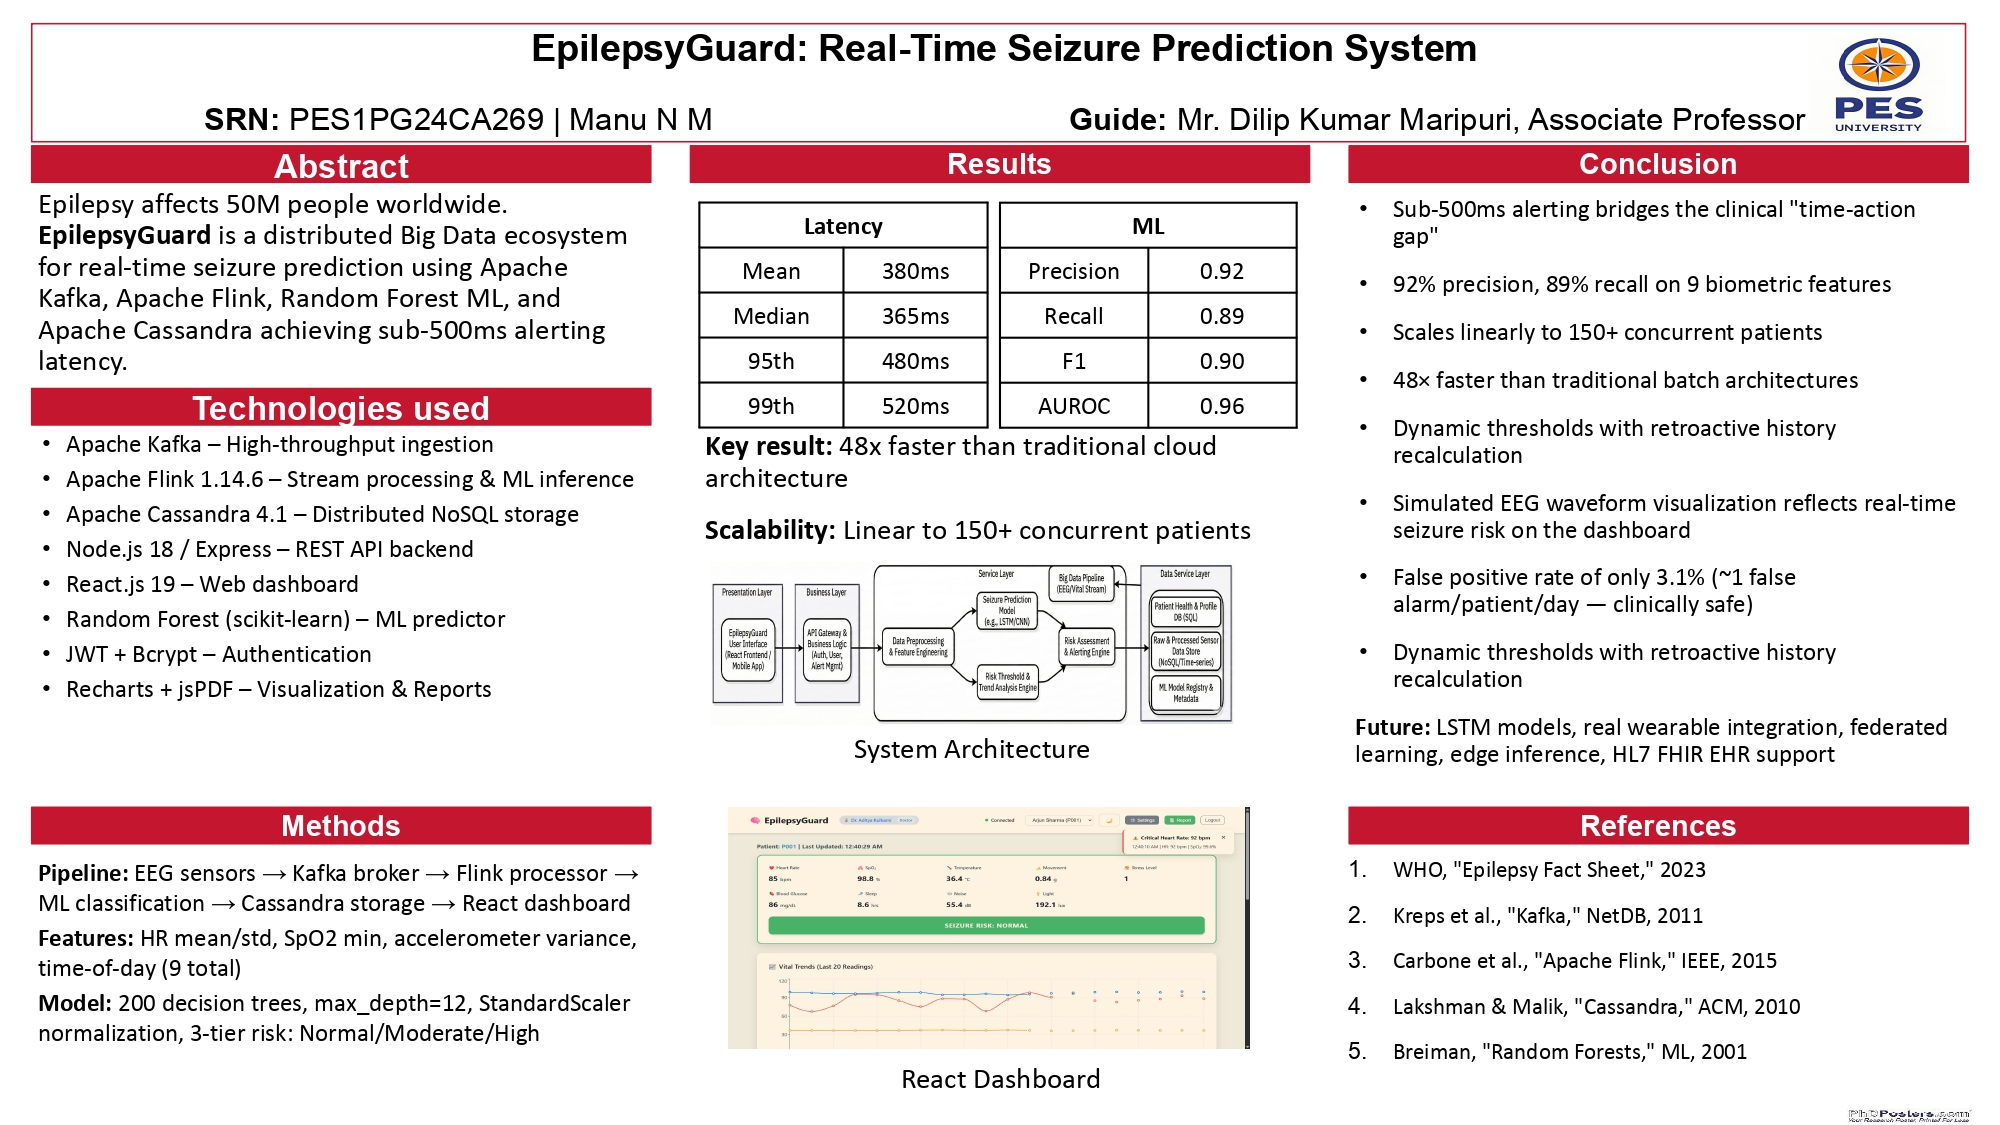
\includegraphics[width=1.0\textwidth]{Poster.jpg}
    \caption{Final project presentation poster.}
    \label{fig:poster}
\end{figure}

\end{document}